\section{Zielsetzung}
In diesem Experiment soll eine Dispersionskurve erfasst werden mittels eines Prismas.

\section{Theorie}
Tritt eine Lichtwelle auf eine Grenzschicht, beispielsweise zwischen zwei Medien, dann kommt es zur Wechselwirkung zwischen der Lichtwelle und den
Elektronen und den Ionenrümpfen des Materials. Dabei wird die Lichtgeschwindigkeit der Lichtwelle und dessen Ausbreitungsrichtung verändert. Dieses
Phänomen wird als \textbf{Brechung} bezeichnet. Mit Hilfe des \textbf{Huygensches Prinzip}, welches besagt, dass jeder Punkt einer bestehenden Welle als
Ausgangspunkt einer kugelförmigen Elementarwelle angesehen werden kann und die einhüllende Welle die Wellenfront beschreibt, kann eine Relation
für den \textbf{Brechungsindex} $n$ hergeleitet werden:
\begin{equation*}
  n=\frac{\sin\alpha}{\sin\beta}
\end{equation*}
$\alpha$ und $\beta$ sind in Abbildung \ref{abb:1} dargestellt.
\begin{figure}
  \centering
  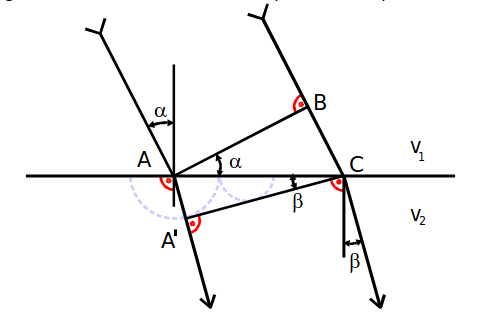
\includegraphics[scale=0.4]{1.png}
  \caption{Darstellung einer gebrochenen Welle an einer Grenzschicht. \cite{Q1}}
  \label{abb:1}
\end{figure}
Der Brechungsindex $n$ beschreibt außerdem die Relation der Lichtgeschwindigkeiten
\begin{equation*}
  n = \frac{v_1}{v_2}
\end{equation*}
dies lässt darauf schließen, dass der Brechungsindex frequenzabhängig sein muss. Die frequenzabhängigkeit des Brechungsindexes wird als \textbf{Dispersion}
bezeichnet. Wenn der Brechungsindex $n$ mit wachsendem $\lambda$ kleiner wird, wird dies als normale Dispersion bezeichnet. Wenn aber der Brechungsindex
bei wachsendem $lambda$ größer wird, wird von einer anormalen Dirpersion gesprochen.

\subsection{Dispersionsgleichung}
Wenn eine Lichtwelle auf eine Grenzschicht trifft, wechselwirkt das elektrische Feld mit den Elektronene und den Ionenrümpfen. Hierbei entstehen mehrere
Kräfte: eine auslenkende, periodische Kraft (durch das elektirsche Feld der eintretenden Welle), eine rücktreibende Kraft (proportional zur Auslenkung), eine
Reinbungskraft (hervorgerufen durch das Medium).
Aus diesen Kräften lässt sich die folgende Differentialgleichung aufstellen:
\begin{equation*}
  \frac{\symup{d^2}\vec{P}_h}{\symup d t^2}+ \frac{f_h}{m_h} \frac{\symup d \vec{P}_h}{\symup d t}+ \frac{a_h}{m_h} \vec{P}_h = \frac{N_q q²_h}{m_h} \vec{E}_0 \symup e^{i \omega t}
\end{equation*}
wobei $\vec{P}_h$ die Polarisation, $m_h$ die Teilchenmasse, $f_h$ die Reibungskonstante, $a_h$ die Federkonstante, $q_h$ die Ladung, $N_h$ die
Ladungsträgerdichte, $E_0$ die Amplitude des elektrischen Feldes der einfallenden Lichtwelle beschreibt und der Index $h$ für das jeweilige Teilchen steht.
Für diese Differentialgleichung ist die Lösung bekannt,
\begin{equation*}
  \vec{P}=\sum\limits_h \frac{1}{\omega_h²-\omega²+i\frac{f_h}{m_h}\omega} \frac{N_q q²_h}{m_h} \vec{E}_0 \symup{e}^{i\omega t} \ \ \ \symup{mit} \ \frac{a_h}{m_h}=\omega².
\end{equation*}
Da die Polarisation in einem Medium der dielektrischen Verschiebung entspricht
\begin{equation*}
  \vec{P} = (\epsilon-1)\epsilon_0 \vec{E}
\end{equation*}
und die Relation $\tilde{n}²=\epsilon$ gilt, kann die Lösung der Differentialgleichung nach dem Brechungindex $n$ umgeformt werden. Außderm muss noch betrachtet
werden, dass $\tilde{n}$ einer komplexen Zahl enspricht, wobei für diesen Versuch nur der Realteil von $\tilde{n}$ von Bedeutung ist. Der Imaginärteil die
Absorptionskonstante beinhaltet. Der reele Anteil $\symup{Re}(\tilde{n})=n$ entspricht dem gesuchten Brechungindex.
Da die Differentialgleichung nur eine Näherung für das Problem beschreibt, müssen zunächst Annahmen für die Gültigkeit dieser gemacht werden. Eine dieser
Annahmen ist, dass die Gleichung nicht in der Nähe der Absortionsfrequenzen durchgeführt wird, also das $\lambda << \lambda_1$ oder $\lambda >> \lambda_1$ gilt,
diese wird in dem Experiment damit erfüllt, dass wir im Bereich des sichtbaren Lichtes liegen und dort keine Absorptionsfreuquenzen des verwendeten Materials liegen.
Mit dieser Bedingung, kann $n²k \approx 0$ angenommen werden. Daraus folgt für den Brechungsindex:
\begin{equation}
  \label{eq:1}
  n²(\lambda)=1+ \frac{N_1 q_1²}{4\pi² c² \epsilon_0 m_1} \frac{\lambda_1²}{{1-\left(\frac{\lambda_1}{\lambda}\right)²}}
\end{equation}
Mittels dieser Formel kann jetzt eine Fallunterscheidung durchgeführt werden:
\begin{itemize}
  \item $\lambda << \lambda_1$: Liegt die Resonanzstelle also über der Messstelle, kann die Gleichung \eqref{eq:1} mittels einer Taylorentwicklung vereinfacht
  werden. Die dabei entstehende Kurve ist in Abbildung \ref{abb:2} b) abgebildet.
  \begin{equation*}
    n²(\lambda) = 1+\frac{N_1 q²_1 \lambda_1²}{4 \pi c² \epsilon_0 m_1} \left(1+\left(\frac{\lambda_1}{\lambda}\right)²+\left(\frac{\lambda_1}{\lambda}\right)⁴+ ...\right)
  \end{equation*}
  mit den Koeffizienten $A_i>0$:
  \begin{equation*}
    n²(\lambda) = A_0 + \frac{A_2}{\lambda²}+\frac{A_4}{\lambda⁴}+...
  \end{equation*}
  \item $\lambda >> \lambda_1$: Liegt die Resonanzstelle unter der Messstelle, kann die Gleichung \eqref{eq:1} erneut mittels einer Taylorentwicklung vereinfacht
  werden. Die dabei entstehende Kurve ist in Abbildung \ref{abb:2} a) abgebildet.
  \begin{equation*}
      n²(\lambda) = 1-\frac{N_1 q¹_1}{4 \pi c² \epsilon_0 m_1} \left(\lambda²+\frac{\lambda⁴}{\lambda_1^2}+\frac{\lambda⁶}{\lambda_1^4}+...\right)
  \end{equation*}
  und mit den Koeffizienten $A'_i>0$:
  \begin{equation*}
    n²(\lambda) = 1-A'_2\lambda²-A'_4\lambda⁴-...
  \end{equation*}
\end{itemize}
\FloatBarrier
\begin{figure}
  \centering
  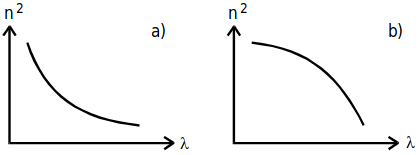
\includegraphics[scale=0.6]{2.png}
  \caption{Dispersionskurven für a) $\lambda >> \lambda_1$ und b) $\lambda << \lambda_1$. \cite{Q1}}
  \label{abb:2}
\end{figure}
\FloatBarrier
\section{Auswertung}
